\documentclass[10pt,twocolumn,letterpaper]{article}
\usepackage[margin=.75in,columnsep=.25in]{geometry}
\usepackage{fontspec,kotex}
\setmainfont{Times New Roman}
\setsansfont{Arial}
\setmainhangulfont{Malgun Gothic}
\setsanshangulfont{Malgun Gothic}
\renewcommand{\abstractname}{초록}
\renewcommand{\refname}{참고문헌}
\renewcommand{\figurename}{그림}
\renewcommand{\tablename}{표}
\usepackage{amsmath,amssymb,graphicx,booktabs,tikz,natbib,xcolor,hyperref}
\hypersetup{colorlinks=true,linkcolor=blue!55!black,citecolor=blue!55!black,urlcolor=blue!55!black}
% Shared colours and TikZ styles for the PGCT papers and slides (requires tikz, xcolor).
\usetikzlibrary{arrows.meta,positioning,calc,fit,backgrounds,shapes.geometric}
\definecolor{pgblue}{HTML}{1F4E9A}
\definecolor{pgsky}{HTML}{DCE7F7}
\definecolor{pgorange}{HTML}{C0504D}
\definecolor{pgsand}{HTML}{FBE9DA}
\definecolor{pggreen}{HTML}{2E7D4F}
\definecolor{pgmint}{HTML}{E2F2E8}
\definecolor{pggrey}{HTML}{6B6B6B}
\definecolor{pglight}{HTML}{F4F4F4}
\tikzset{
  pg/.style={font=\sffamily\small},
  stage/.style={draw=pgblue,line width=.8pt,rounded corners=3pt,fill=white,align=center,
                minimum height=1.25cm,text width=2.7cm,inner sep=3pt},
  card/.style={draw=pggrey,rounded corners=2pt,fill=white,align=center,inner sep=2.5pt,font=\sffamily\scriptsize},
  box/.style={draw=pgblue,line width=.8pt,rounded corners=3pt,fill=white,align=center,inner sep=4pt},
  flow/.style={-{Stealth[length=2.4mm]},line width=.9pt,draw=pgblue},
  flowg/.style={-{Stealth[length=2.2mm]},line width=.8pt,draw=pggrey},
  flowo/.style={-{Stealth[length=2.4mm]},line width=.9pt,draw=pgorange},
  band/.style={rounded corners=5pt,inner sep=7pt},
  num/.style={circle,fill=pgblue,text=white,font=\sffamily\bfseries\scriptsize,inner sep=1.2pt,minimum size=4mm},
  lbl/.style={font=\sffamily\scriptsize,text=pggrey,align=center},
}
\newcommand{\stagetitle}[1]{{\bfseries\color{pgblue}#1}}

% Shared verbatim by the English and Korean manuscripts. Numbers follow invocation order.
\newcommand{\ModelEquation}{\begin{equation}\label{eq:model}
 \widehat r_i(q;\psi_i)=\operatorname{MLP}_{\psi_i}
 [u_t,\operatorname{onehot}(a_t),u_{t+1}],\quad u_t=P(o_{i,t}).
\end{equation}}
\newcommand{\RewardLossEquation}{\begin{equation}\label{eq:rloss}
 \mathcal L_i^r=\mathbb E_{(q,r_i)\sim\mathcal B_i^{\rm mix}}
 [(\widehat r_i(q;\psi_i)-r_i)^2].
\end{equation}}
\newcommand{\ProbeEquation}{\begin{equation}\label{eq:probe}
 \mathcal Q_{ij}^{u}=\mathcal E_i^{u}\cup\mathcal E_j^{u}
 \cup M\big(\mathcal E_i^{u}\cup\mathcal E_j^{u}\big).
\end{equation}}
\newcommand{\DistanceEquation}{\begin{equation}\label{eq:distance}
 D_{ij}^{u}=\frac{\sum_{q\in\mathcal Q_{ij}^{u}}|\widehat r_i^{\,u}(q)-\widehat r_j^{\,u}(q)|}
 {\sum_{q\in\mathcal Q_{ij}^{u}}\big(|\widehat r_i^{\,u}(q)|+|\widehat r_j^{\,u}(q)|\big)}.
\end{equation}}
\newcommand{\ApprovalEquation}{\begin{align}\label{eq:approval}
 \bar D_{ij}&\leftarrow (1-\beta)\bar D_{ij}+\beta D_{ij}^{u},\quad\beta=0.35,\\
 B_{ij}&=\mathbf 1[i\ne j,\ n_{ij}\ge3,\ \bar D_{ij}<0.5,\ m_i^{u}=m_j^{u}=1].\nonumber
\end{align}}
\newcommand{\DonorEquation}{\begin{align}\label{eq:donor}
 C_{ij}^{u}&=\mathbf1[\exists t\text{ in rollout }u:\|p_{i,t}-p_{j,t}\|_\infty\le3],\\
 \mathcal G_i^u&=\{j\ne i:C_{ij}^u B_{ij}=1\}.\nonumber
\end{align}}
\newcommand{\MaxEquation}{\begin{align}\label{eq:max}
 b_{i,t}&=\min\{c,[\max_{j\in\mathcal G_i^u}V_j(\tilde h_{i,t}^{\,j})-V_i(h_{i,t})]_+\},\\
 f_{i,t}&=V_i(h_{i,t})+w_t b_{i,t}.\nonumber
\end{align}}
\newcommand{\GAEEquation}{\begin{align}\label{eq:gae}
 \delta_{i,t}^{f}&=r_{i,t}+\gamma(1-d_t)f_{i,t+1}+\gamma z_{i,t}^{f}-f_{i,t},\\
 A_{i,t}^{f}&=\delta_{i,t}^{f}+\gamma\lambda_f(1-d_t)A_{i,t+1}^{f}.\nonumber
\end{align}}
\newcommand{\BlendEquation}{\begin{align}\label{eq:blend}
 \Delta_{i,t}&=w_t(A_{i,t}^{f}-A_{i,t}^{\rm self}),\\
 s_i&=\min\!\left(1,\frac{\operatorname{std}_t A_{i,t}^{\rm self}}
 {\max(\operatorname{std}_t\Delta_{i,t},10^{-8})}\right),\nonumber\\
 A_{i,t}^{\rm PGCT}&=A_{i,t}^{\rm self}+\eta s_i\Delta_{i,t},\qquad \eta=0.5.\nonumber
\end{align}}
\newcommand{\PPOEquation}{\begin{align}\label{eq:ppo}
 \rho_{i,t}(\theta_i)&=\pi_{\theta_i}(a_{i,t}\mid h_{i,t})/\pi_{\theta_i^{\rm old}}(a_{i,t}\mid h_{i,t}),\\
 L_i^\pi&=\mathbb E_t[\min\{\rho_{i,t}\widetilde A_{i,t},
 \operatorname{clip}(\rho_{i,t},1-\epsilon,1+\epsilon)\widetilde A_{i,t}\}],\nonumber\\
 R_{i,t}^{\rm self}&=A_{i,t}^{\rm self}+V_i^{\rm old}(h_{i,t}).\nonumber
\end{align}}
\newcommand{\BoundEquation}{\begin{equation}\label{eq:bound}
 \|\Delta A\|_\infty\le\left(1+\frac{\gamma(1-\lambda)}{1-\gamma\lambda}\right)\|\Delta f\|_\infty.
\end{equation}}

\setlength{\emergencystretch}{2em}
\linespread{1.08}
\newcommand{\pending}{\textcolor{pgorange}{\textit{진행 중}}}
\title{Probe-Gated Critic Transfer:\\개인 보상 응답을 이용한 잠재 팀 발견}
\author{익명 제출본}
\date{}
\begin{document}
\maketitle

\begin{abstract}
많은 다중 에이전트 시스템에서 에이전트들은 같은 공간을 쓰지만 같은 목표를 갖지는 않는다. 한 창고의 로봇들이 서로 다른 요청 목록을 처리할 수 있고, 에이전트는 가까이 있다는 사실만으로 어떤 이웃이 같은 과제를 하는지 알 수 없다. 이 논문은 완전 분산 다중 팀 강화학습에서 \emph{온라인 잠재 팀 발견}을 다룬다. 각 에이전트는 자기 관측과 자기 개인 보상만 보고, 팀 라벨은 주어지지 않으며, 물리적으로 가까울 때만 제한된 정보를 주고받는다. 우리는 Probe-Gated Critic Transfer(PGCT)를 제안한다. 각 에이전트는 자기 보상을 예측하는 작은 모델을 학습한다. 두 에이전트가 만나면 공통 Reward Probe, 즉 공개 보상 사건 묶음에 두 예측기를 함께 적용하고, 응답 차이를 정규화된 거리로 비교한다. 거리가 반복해서 낮고 두 에이전트 모두 자기 보상 경험이 충분하면 잠재 팀원으로 승인한다. 증거가 부족하면 판정을 보류한다. 발견한 관계가 학습에 유용한지 확인하기 위해, 승인된 팀원의 Critic으로 받는 에이전트 자신의 관측 이력을 평가한다. 그 양의 가치 상승분은 마스크와 크기 제한을 둔 Max-GAE advantage를 통해 Actor에만 반영되고, 모든 Critic은 자기 return만 학습한다. 개인 보상을 쓰는 6 에이전트·2 팀 창고 과제에서, 발견 구성요소는 약 0.25M step부터 같은 팀과 다른 팀 쌍을 구분했다(평균 응답 거리 0.25 대 0.99). 5M step 동안 승인된 팀원 접근의 93.7\%가 실제 팀원에게 향했다. 통합 방법의 학습 비교는 진행 중이며, 결과는 진행 중으로 표시한다.
\end{abstract}

\section{서론}
다중 에이전트 강화학습(MARL)의 협력 방법은 대개 협력할 집단을 미리 안다고 가정한다. 팀 공동 보상, 중앙 Critic, 파라미터 공유는 모두 어떤 에이전트끼리 한 팀인지 전제한다 \citep{mappo,seps}. 실제로는 이 가정을 쓸 수 없는 경우가 많다. 한 창고 안에서 여러 로봇 팀이 각자의 요청 목록을 처리하고 각자의 목적지로 배송할 수 있다. 에이전트는 이웃을 볼 수 있지만, 가까이 있다는 사실만으로 그 이웃이 같은 과제를 하는지는 알 수 없다. 가치 정보를 무차별하게 공유하면 서로 다른 목표로 학습한 추정이 섞인다. 반대로 전혀 공유하지 않으면 이미 과제를 익힌 팀원의 도움을 받을 수 없다.

그래서 두 질문을 던진다. \textbf{Q1(발견):} 에이전트가 자기 경험과 국소 통신만으로 잠재 팀원을 온라인에서 찾을 수 있는가? \textbf{Q2(활용):} 팀원을 찾았을 때 그 가치 정보가 학습에 도움이 되는가? 이 논문의 중심은 Q1이다. Q2는 발견한 관계가 실제 학습에 쓸모 있는지 검증하는 역할을 한다.

Q1에 먼저 떠오르는 신호는 정책 유사도다. 하지만 같은 과제의 에이전트라도 학습 중에는 정책이 다를 수 있고, 다른 과제의 에이전트라도 둘 다 거의 무작위로 움직이면 비슷해 보인다. 우리는 과제를 정의하는 양, 즉 보상을 쓴다. 같은 팀의 에이전트는 같은 규칙으로 보상을 받으므로, 같은 사건은 두 에이전트 모두에게 보상이 된다. 다른 팀의 에이전트는 다른 사건에서 보상을 받는다. 각 에이전트는 보상 값을 공유하지 않고도 자기 보상으로 이 규칙을 학습할 수 있다. 그다음 두 에이전트는 공통 공개 사건에 대해 각자의 보상 예측기가 무엇이라고 답하는지 비교한다. 여기에는 세 가지 어려움이 있다. 보상 사건은 드물다. 관측에는 주고받으면 안 되는 과제 고유 채널이 있다. 그리고 보상 경험이 없는 에이전트는 비교할 보상 규칙 자체가 없다.

\paragraph{기여.}
\begin{itemize}\setlength\itemsep{1pt}
\item 개인 보상, 팀 라벨 없음, 접촉으로 제한된 통신이라는 조건에서 완전 분산 다중 팀 MARL의 온라인 잠재 팀 발견 문제를 정의한다.
\item 발견을 위한 보상 응답 Reward Probe 검정을 제안한다. 각 에이전트는 공개 전이에서 자기 보상을 예측하는 모델을 학습한다. 두 에이전트가 만나면 공통 보상 사건 probe에서 예측을 비교하고, 척도에 의존하지 않는 거리를 계산한다. 일치가 지속되면 승인하고, 자기 보상 증거가 부족한 에이전트는 판정을 보류한다. 비교에는 접촉 시점에 실제로 존재한 정보만 들어간다.
\item 발견한 관계를 선택적 팀원 Critic 접근으로 활용한다. 승인된 팀원의 Critic이 받는 에이전트 자신의 이력을 평가하고, 그 양의 상승분이 마스크와 크기 제한을 둔 Max-GAE 항으로 Actor advantage를 바꾼다. 각 Critic은 자기 return만 목표로 하며, 승인된 팀원이 없으면 방법은 독립 PPO와 정확히 같아진다.
\item 창고 과제에서 근거를 보고한다. 발견 로그, 발견 규칙의 오프라인 재생, 팀 관계가 팀원 가치에 왜 중요한지 보여 주는 반사실 점검이다. 아직 진행 중인 학습 비교를 위한 분기 실험 절차도 제시한다.
\end{itemize}

\section{관련 연구}
\paragraph{독립 학습과 공유 학습.}
독립 학습자는 자기 목표를 최적화하며, 협력 MARL에서도 여전히 강한 기준선이다 \citep{tan,ippo,benchmark}. PPO와 일반화 advantage 추정(GAE)은 이런 학습자의 표준 구성요소다 \citep{ppo,gae,mappo}. Shared Experience Actor-Critic은 협력하는 에이전트끼리 경험을 공유한다 \citep{seac}. 선택적 파라미터 공유는 에이전트를 묶은 뒤 파라미터를 공유한다 \citep{seps}. 완전 분산 actor-critic 방법은 네트워크로 연결된 에이전트가 공통 Critic에 합의하게 한다 \citep{fdmarl}. 이 방법들은 공통 목표를 가진 집단이 주어지거나, 모든 에이전트가 하나의 목표를 공유한다고 가정한다. PGCT는 개인 보상에서 집단을 추론하고, Actor와 Critic을 각자 따로 유지한다.

\paragraph{다른 에이전트 모델링.}
에이전트 모델링은 다른 에이전트의 목표, 유형, 정책 같은 성질을 추론한다 \citep{modelling}. Ad hoc 팀워크는 사전 조율 없이 모르는 팀원과 협력하는 문제를 다룬다 \citep{adhoc}. 우리가 추론하는 대상은 더 좁다. 다른 에이전트가 같은 규칙으로 보상받는지다. 추론에는 자기 보상 예측기와 공개 사건에 대한 상대의 예측만 쓰며, 상대 정책의 모델은 필요하지 않다.

\paragraph{여러 가치함수의 결합.}
일반화 정책 개선은 여러 정책의 가치함수를 최댓값으로 결합한다 \citep{gpi}. MAMBA는 여러 oracle 가치의 상태별 최댓값을 GAE 형태의 추정기에 넣고, oracle 가치를 학습자의 상태 분포에서 추정할 때 개선 보장을 준다 \citep{mamba}. 우리의 Max-GAE 항은 이 결합 방식을 따른다. 그러나 전제는 성립하지 않는다. 팀원 Critic은 팀원 자신의 이력에서 학습되었고, 받는 에이전트의 이력에서 평가된다. rollout으로 다시 추정한 oracle 가치가 아니다. 따라서 성능 보장을 주장하지 않으며, 팀원 가치는 효과를 실험으로 측정해야 하는 Actor 보조 신호로 다룬다.

\section{문제 설정}
부분 관측 환경의 에이전트 $N$개를 생각한다. 에이전트 $i$는 관측 $o_{i,t}$를 받고 행동 $a_{i,t}$를 하며 자기 스칼라 보상 $r_{i,t}$를 받는다. 각 에이전트에는 숨은 팀 라벨 $z_i$가 있고, 같은 팀의 에이전트는 같은 규칙으로 보상받는다. $z_i=z_j$이면 두 에이전트를 \emph{잠재 팀원}이라 한다. 라벨은 평가와 oracle 기준선에만 쓴다.

\paragraph{정보 모델.}
각 에이전트는 자기 recurrent Actor와 Critic을 갖는다. 에이전트 $i$와 $j$는 rollout $u$ 중 어느 step에서든 Chebyshev 거리 3 이내로 가까워졌을 때만 통신할 수 있다.
\DonorEquation
접촉했을 때 주고받을 수 있는 것은 공개 사건 view, 그 view에 대한 예측 보상, Critic 가중치다. 보상 값, 팀 라벨, Actor 가중치, 개인 궤적은 주고받지 않는다. 공개 투영 $P$는 과제 고유 관측 채널(요청 선반, 자기 팀 목적지)과 절대 좌표를 지운다. 구현에서 $P(o)$는 자기 상태 특징 6개와 반경 2 이내의 물리 격자 채널 11개를 남긴 281차원 view다. Actor와 Critic은 좌표 두 칸만 0으로 바꾼 전체 의미 관측을 쓴다.

\paragraph{목표.}
각 에이전트는 만난 에이전트에 대해 관계 $\mathbf 1[z_i=z_j]$를 추정하고, 증거가 부족하면 판정을 보류해야 한다. 그리고 자기 보상이나 Critic 목표를 바꾸지 않은 채 이 추정을 자기 학습 개선에 써야 한다.

\section{Probe-Gated Critic Transfer}
\begin{figure*}[t]
\centering\resizebox{.97\textwidth}{!}{% Figure 1: overall PGCT pipeline of one agent i (all steps are local to i; peers only exchange on contact).
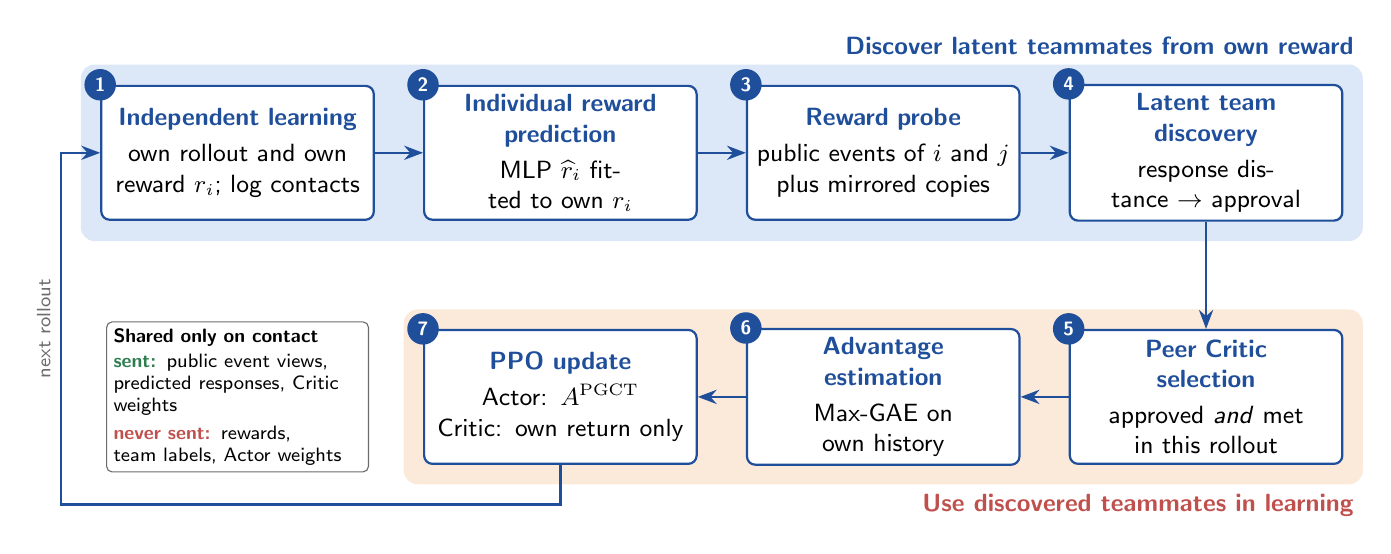
\begin{tikzpicture}[pg]
\tikzset{stage/.append style={text width=3.25cm,minimum height=1.7cm}}
\node[stage] (s1) at (0,0)     {\stagetitle{Independent learning}\\[2pt]own rollout and own\\reward $r_i$; log contacts};
\node[stage] (s2) at (4.1,0)   {\stagetitle{Individual reward}\\\stagetitle{prediction}\\[2pt]MLP $\widehat r_i$ fitted to own $r_i$};
\node[stage] (s3) at (8.2,0)   {\stagetitle{Reward probe}\\[2pt]public events of $i$ and $j$\\plus mirrored copies};
\node[stage] (s4) at (12.3,0)  {\stagetitle{Latent team}\\\stagetitle{discovery}\\[2pt]response distance $\to$ approval};
\node[stage] (s5) at (12.3,-3.1){\stagetitle{Peer Critic}\\\stagetitle{selection}\\[2pt]approved \emph{and} met\\in this rollout};
\node[stage] (s6) at (8.2,-3.1) {\stagetitle{Advantage}\\\stagetitle{estimation}\\[2pt]Max-GAE on own history};
\node[stage] (s7) at (4.1,-3.1) {\stagetitle{PPO update}\\[2pt]Actor: $A^{\rm PGCT}$\\Critic: own return only};
\foreach \k [count=\n] in {s1,s2,s3,s4,s5,s6,s7} {\node[num] at (\k.north west) {\n};}
\draw[flow] (s1) -- (s2); \draw[flow] (s2) -- (s3); \draw[flow] (s3) -- (s4);
\draw[flow] (s4) -- (s5); \draw[flow] (s5) -- (s6); \draw[flow] (s6) -- (s7);
\draw[flow] (s7.south) -- ++(0,-0.5) -| ($(s1.west)+(-0.5,0)$)
  node[lbl,pos=.75,rotate=90,above]{next rollout} -- (s1.west);
\node[card,text width=3.15cm,align=left,font=\sffamily\scriptsize] (info) at (0,-3.1)
  {\textbf{Shared only on contact}\\[1pt]
   \textcolor{pggreen}{\textbf{sent:}} public event views,\\ predicted responses, Critic weights\\[2pt]
   \textcolor{pgorange}{\textbf{never sent:}} rewards,\\ team labels, Actor weights};
\begin{scope}[on background layer]
\node[band,fill=pgsky,fit=(s1)(s4),label={[font=\sffamily\small\bfseries,text=pgblue,anchor=south east]north east:Discover latent teammates from own reward}] {};
\node[band,fill=pgsand,fit=(s5)(s7),label={[font=\sffamily\small\bfseries,text=pgorange,anchor=north east]south east:Use discovered teammates in learning}] {};
\end{scope}
\end{tikzpicture}
}
\caption{한 에이전트의 PGCT 전체 절차. 2--4단계는 자기 보상에서 잠재 팀원을 찾고, 5--7단계는 승인된 팀원을 Actor advantage로만 활용한다. 모든 계산은 국소적이며, 팀원끼리는 접촉했을 때만 공개 사건 view, 예측 응답, Critic 가중치를 주고받는다.}\label{fig:architecture}
\end{figure*}

그림~\ref{fig:architecture}는 PGCT 한 번의 update를 요약한다. 1--4단계가 Q1, 5--7단계가 Q2에 해당한다.

\subsection{개인 보상 예측}
각 에이전트는 공개 전이 $q=(u_t,a_t,u_{t+1})$에서 자기 보상을 예측하는 다층 퍼셉트론을 학습한다.
\ModelEquation
입력은 $281+5+281=567$차원이고, 은닉층은 ReLU 128개와 64개다. 각 에이전트는 최근 전이 20{,}000개와, 이와 별도로 최근 보상 사건 512개를 저장한다. 사건은 자기 보상이 $r_i\ge0.5$인 전이이며, 이 과제에서는 배송과 선반 반납이다. 사건은 전이의 0.5\% 미만이므로, 학습 batch의 4분의 1을 사건 버퍼에서 뽑는다. 손실은 다음과 같다.
\RewardLossEquation
예측기는 PPO update 5번마다 Adam으로 50 step 학습한다(batch 256, 학습률 $10^{-3}$). 공개 view는 과제 고유 정보를 숨기므로, 같은 공개 전이가 보상일 수도 아닐 수도 있다. 이때 회귀는 보상의 조건부 평균을 배우며, 비교하는 양이 바로 이것이다.

\subsection{Reward Probe}
rollout $u$ 동안 $i$와 $j$가 만났다면, 두 에이전트는 다음 공통 probe 집합을 만든다.
\ProbeEquation
$\mathcal E_i^u$는 rollout $u$가 시작되기 전에 기록된 에이전트 $i$의 최근 자기 사건 32개의 공개 view이고, $M$은 view와 회전 행동을 좌우로 뒤집는다. probe는 코드와 같이 중복을 허용해 이어 붙인다. 좌우 대칭은 한 팀의 사건만으로는 던질 수 없는 반사실 질문을 만든다. 모서리 배치에서 한 목적지의 배송 장면을 뒤집으면 다른 목적지의 배송처럼 보인다. 보상 값은 probe에 들어가지 않는다.

\paragraph{인과적 스냅샷.}
비교는 rollout이 끝난 뒤 이루어지지만, 두 에이전트는 rollout 초반에 만났을 수도 있다. 접촉 시점에 존재한 정보만 쓰기 위해, 각 에이전트는 rollout $u$를 시작할 때 사건 probe, 성숙 여부, 예측기 버전을 고정한다. 예측기는 rollout이 끝난 뒤에만 다시 학습되므로, 고정된 버전이 곧 rollout 동안 쓰인 예측기다. rollout $u$의 비교는 이 고정본으로 하고, 예측기 재학습보다 먼저 수행한다.

\begin{figure*}[t]
\centering\resizebox{.97\textwidth}{!}{% Figure 2: reward-based team discovery for one contacted pair (i, j). Bars are illustrative, not data.
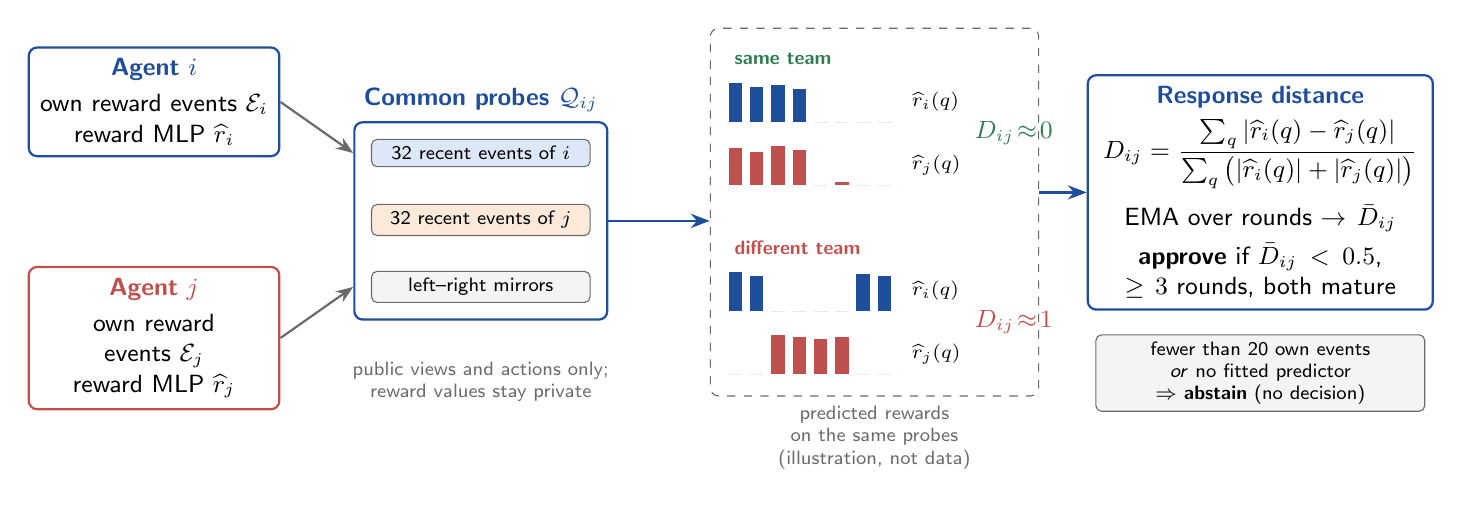
\begin{tikzpicture}[pg]
\def\pgbars#1#2#3#4{% colour, x0, y0, list of heights
  \foreach \h [count=\k] in {#4} {\fill[#1] (#2+0.27*\k-0.27,#3) rectangle ++(0.17,0.55*\h);}}
% agents
\node[box,text width=2.9cm] (ai) at (0,1.5) {\stagetitle{Agent $i$}\\[2pt]own reward events $\mathcal E_i$\\reward MLP $\widehat r_i$};
\node[box,text width=2.9cm,draw=pgorange] (aj) at (0,-1.5) {{\bfseries\color{pgorange}Agent $j$}\\[2pt]own reward events $\mathcal E_j$\\reward MLP $\widehat r_j$};
% probe set
\node[card,text width=2.6cm,fill=pgsky] (ei) at (4.15,0.85) {32 recent events of $i$};
\node[card,text width=2.6cm,fill=pgsand] (ej) at (4.15,0.0) {32 recent events of $j$};
\node[card,text width=2.6cm,fill=pglight] (mi) at (4.15,-0.85) {left--right mirrors};
\node[box,fill=none,fit=(ei)(ej)(mi),inner sep=6pt,label={[font=\sffamily\small\bfseries,text=pgblue]above:Common probes $\mathcal Q_{ij}$}] (Q) {};
\draw[flowg] (ai.east) -- (Q.west|-ei);
\draw[flowg] (aj.east) -- (Q.west|-mi);
\node[lbl,text width=3.3cm] at (4.15,-2.05) {public views and actions only;\\reward values stay private};
% response panels (illustrative)
\begin{scope}[shift={(7.3,0.45)}]
  \node[font=\sffamily\scriptsize\bfseries,text=pggreen,anchor=west] at (-0.05,1.6) {same team};
  \pgbars{pgblue}{0}{0.8}{.9,.8,.85,.75,0,0,0,0}
  \pgbars{pgorange}{0}{0}{.85,.75,.9,.8,0,.05,0,0}
  \node[font=\sffamily\scriptsize,anchor=west] at (2.2,1.05) {$\widehat r_i(q)$};
  \node[font=\sffamily\scriptsize,anchor=west] at (2.2,0.25) {$\widehat r_j(q)$};
  \node[font=\sffamily\small\bfseries,text=pggreen,anchor=west] at (3.0,0.65) {$D_{ij}\!\approx\!0$};
\end{scope}
\begin{scope}[shift={(7.3,-1.95)}]
  \node[font=\sffamily\scriptsize\bfseries,text=pgorange,anchor=west] at (-0.05,1.6) {different team};
  \pgbars{pgblue}{0}{0.8}{.9,.8,0,0,0,0,.85,.8}
  \pgbars{pgorange}{0}{0}{0,0,.9,.85,.8,.85,0,0}
  \node[font=\sffamily\scriptsize,anchor=west] at (2.2,1.05) {$\widehat r_i(q)$};
  \node[font=\sffamily\scriptsize,anchor=west] at (2.2,0.25) {$\widehat r_j(q)$};
  \node[font=\sffamily\small\bfseries,text=pgorange,anchor=west] at (3.0,0.65) {$D_{ij}\!\approx\!1$};
\end{scope}
\node[draw=pggrey,dashed,rounded corners=3pt,fit={(7.1,2.4)(11.2,-2.2)},inner sep=1pt,
      label={[lbl,text width=4cm]below:predicted rewards on the same probes\\(illustration, not data)}] (R) {};
\draw[flow] (Q.east) -- (R.west|-Q.east);
% decision
\node[box,text width=4.1cm] (dec) at (14.05,0.35) {\stagetitle{Response distance}\\[3pt]
  $D_{ij}=\dfrac{\sum_q|\widehat r_i(q)-\widehat r_j(q)|}{\sum_q\big(|\widehat r_i(q)|+|\widehat r_j(q)|\big)}$\\[5pt]
  EMA over rounds $\to\bar D_{ij}$\\[3pt]
  \textbf{approve} if $\bar D_{ij}<0.5$,\\ $\ge3$ rounds, both mature};
\draw[flow] (R.east|-dec.west) -- (dec.west);
\node[card,text width=4.0cm,anchor=north,fill=pglight,font=\sffamily\scriptsize] at ($(dec.south)+(0,-0.3)$)
  {fewer than 20 own events \emph{or} no fitted predictor\\$\Rightarrow$ \textbf{abstain} (no decision)};
\end{tikzpicture}
}
\caption{만난 두 에이전트의 보상 기반 팀 발견. 두 예측기가 같은 공개 probe에 답한다. 같은 팀은 같은 probe에 보상을 주므로 거리가 0에 가깝다. 다른 팀은 대칭 probe를 포함해 서로 겹치지 않는 probe에 보상을 주므로 거리가 1에 가깝다. 막대는 설명용이며 실험 데이터가 아니다. 자기 보상 사건이 부족한 에이전트는 판정을 보류한다.}\label{fig:discovery}
\end{figure*}

\subsection{응답 거리와 팀 발견}
두 예측기는 같은 probe를 평가한다(그림~\ref{fig:discovery}). 응답 차이는 다음과 같다.
\DistanceEquation
두 예측기가 모두 0이라고 답한 probe는 분자와 분모 어디에도 더해지지 않는다. 따라서 정보 없는 probe가 많아도 거리가 희석되지 않는다. 분모가 $10^{-8}$보다 작으면 비교를 보류한다. 에이전트는 자기 사건을 20개 이상 겪었고, 예측기가 학습되었으며, 자기 최근 사건에 대한 평균 예측이 0.3 이상일 때 \emph{성숙}했다고 본다($m_i^u=1$). 쌍은 5 update마다, 두 에이전트가 모두 성숙했을 때만 비교한다. 거리는 비교 round에 걸쳐 평활하고, 쌍은 다음 규칙으로 승인한다.
\ApprovalEquation
$n_{ij}$는 두 예측기가 모두 새 경험으로 다시 학습된 round의 수다. 승인은 대칭이며 접촉이 끊겨도 유지된다. 예전 승인은 두 에이전트가 다시 만났을 때만 쓰인다. 문턱 0.5는 응답 질량의 대부분이 겹친다는 뜻이며, 실험 결과에 맞춰 조정하지 않고 미리 정했다. 이 판정에는 팀 라벨이 쓰이지 않는다.

\subsection{선택적 팀원 Critic 접근}
rollout $u$에서 에이전트 $i$의 donor 집합은 다음과 같다.
\begin{equation}\label{eq:donorset}
\mathcal G_i^u=\{j\ne i: C_{ij}^u=1,\ B_{ij}=1\}.
\end{equation}
donor Critic 가중치는 rollout $u$ 동안 쓰인 가중치이며 접촉 시 전달받는다. update 동안에는 고정한다. 에이전트 $i$는 자기 관측 열을 각 donor Critic에 다시 넣어 donor별 recurrent 상태 $\tilde h^{\,j}_{i,t}$를 만든다. donor의 hidden 상태는 전달하지 않는다. 재생은 rollout 경계에서 0 상태로 시작하고 episode가 끝나면 초기화된다. 관측 8개가 지나거나 첫 초기화가 일어나기 전에는 재생 가치가 아직 믿을 만하지 않으므로, 마스크 $w_t=0$으로 제외한다.

\subsection{Max-GAE advantage 추정}
donor 집합이 비어 있지 않으면 양의 상승분과 결합 가치는 다음과 같다.
\MaxEquation
상한 $c$는 선택 사항이며 기본값은 $c=+\infty$다. GAE 재귀는 trainer의 종료와 시간 제한 처리를 그대로 따른다.
\GAEEquation
$d_t$는 episode 종료 표시이고, $z^f_{i,t}$는 시간 제한으로 끝난 관측의 가치다(그 밖에는 0). 자기 advantage $A^{\rm self}$는 $f$ 대신 $V_i$로 같은 재귀를 계산한다. $\gamma=0.99$, $\lambda_f=\lambda=0.95$일 때 Actor advantage는 다음과 같다.
\BlendEquation
그림~\ref{fig:critic}이 이 계산을 보여 준다. 두 가지가 중요하다. 첫째, 마스크는 $b$만이 아니라 advantage 차이 $\Delta$에 적용한다. $b$만 가리면 미래 상승분이 GAE 재귀를 통해 초기 구간으로 새어 들어온다. 둘째, 계수 $s_i\le1$은 큰 보조 항을 자기 advantage 크기로 줄이지만, 작은 항을 키우지는 않는다. 이 과제에서 뒤처진 에이전트의 원래 차이는 $\operatorname{std}A^{\rm self}$의 2.6--12배였다. $s_i$가 없으면 PPO의 advantage 정규화 때문에 결과가 $\eta$와 거의 무관해진다.

\begin{figure*}[t]
\centering\resizebox{.97\textwidth}{!}{% Figure 3: selective peer Critic use by receiver i (local computation; peer Critic weights received on contact).
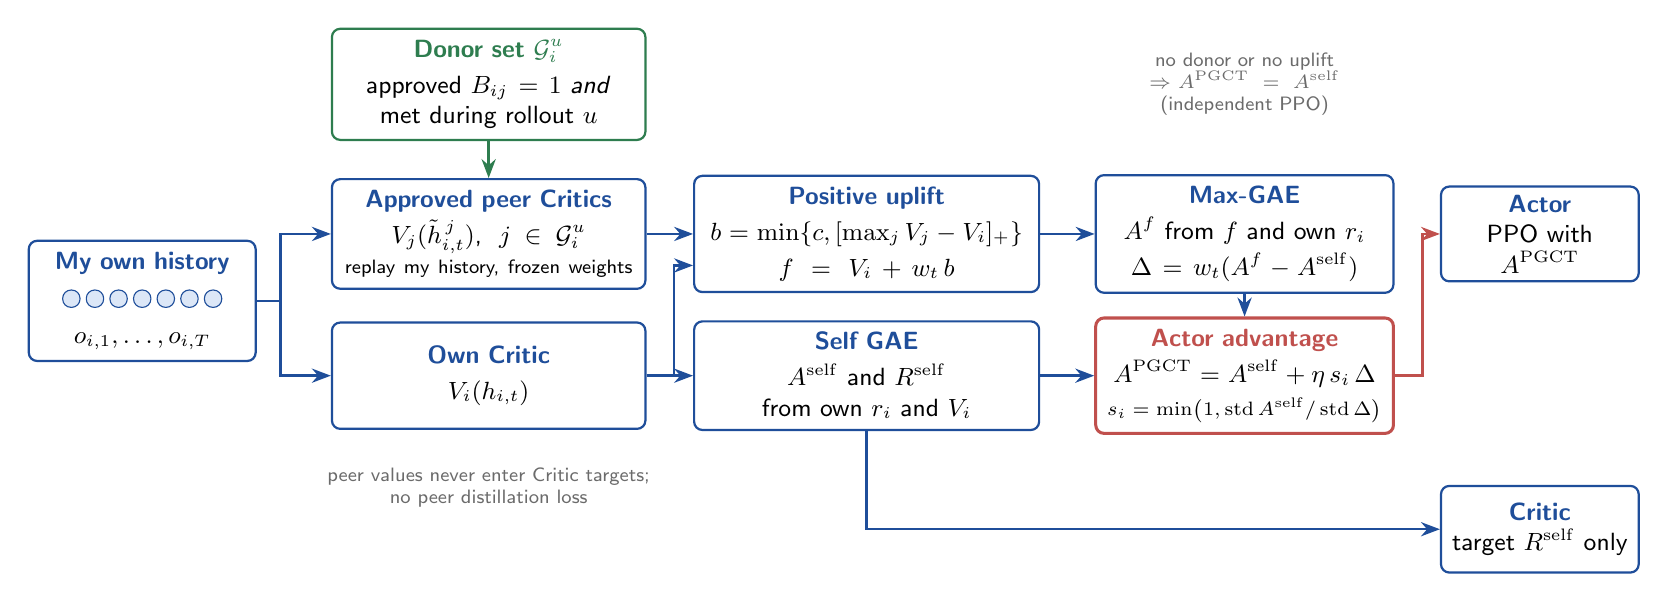
\begin{tikzpicture}[pg]
\tikzset{box/.append style={minimum height=1.35cm}}
% observation stream
\node[box,text width=2.6cm] (obs) at (0,0.8) {\stagetitle{My own history}\\[3pt]
  \tikz{\foreach \k in {0,...,6}{\draw[pgblue,fill=pgsky] (0.3*\k,0) rectangle ++(0.22,0.22);}}\\[2pt]
  $o_{i,1},\dots,o_{i,T}$};
% donor set and critics
\node[box,text width=3.7cm,draw=pggreen] (gate) at (4.4,3.55) {{\bfseries\color{pggreen}Donor set $\mathcal G_i^u$}\\[2pt]
  approved $B_{ij}=1$ \emph{and}\\ met during rollout $u$};
\node[box,text width=3.7cm] (peer) at (4.4,1.65) {\stagetitle{Approved peer Critics}\\[2pt]
  $V_j(\tilde h^{\,j}_{i,t})$, \ $j\in\mathcal G_i^u$\\{\scriptsize replay my history, frozen weights}};
\node[box,text width=3.7cm] (own) at (4.4,-0.15) {\stagetitle{Own Critic}\\[2pt]$V_i(h_{i,t})$};
\draw[flow] (obs.east) -- ++(0.3,0) |- (peer.west);
\draw[flow] (obs.east) -- ++(0.3,0) |- (own.west);
\draw[flow,draw=pggreen] (gate) -- (peer);
% uplift, self GAE, Max-GAE, blend
\node[box,text width=4.1cm] (b) at (9.2,1.65) {\stagetitle{Positive uplift}\\[2pt]
  $b=\min\{c,[\max_j V_j-V_i]_+\}$\\[2pt] $f=V_i+w_t\,b$};
\node[box,text width=4.1cm] (af) at (9.2,-0.15) {\stagetitle{Self GAE}\\[2pt]$A^{\rm self}$ and $R^{\rm self}$\\from own $r_i$ and $V_i$};
\draw[flow] (peer) -- (b);
\draw[flow] (own.east) -- ++(0.35,0) |- ($(b.west)+(0,-0.4)$);
\draw[flow] (own) -- (af);
\node[box,text width=3.5cm] (mg) at (14.0,1.65) {\stagetitle{Max-GAE}\\[2pt]$A^{f}$ from $f$ and own $r_i$\\[2pt]
  $\Delta=w_t(A^f-A^{\rm self})$};
\draw[flow] (b) -- (mg);
\node[box,text width=3.5cm,draw=pgorange,line width=1.1pt] (blend) at (14.0,-0.15) {{\bfseries\color{pgorange}Actor advantage}\\[2pt]
  $A^{\rm PGCT}=A^{\rm self}+\eta\,s_i\,\Delta$\\[1pt] {\scriptsize $s_i=\min\!\big(1,\operatorname{std}A^{\rm self}/\operatorname{std}\Delta\big)$}};
\draw[flow] (mg) -- (blend);
\draw[flow] (af) -- (blend);
% updates
\node[stage,text width=2.3cm,minimum height=1.1cm] (actor) at (17.75,1.65) {\stagetitle{Actor}\\PPO with $A^{\rm PGCT}$};
\node[stage,text width=2.3cm,minimum height=1.1cm] (critic) at (17.75,-2.1) {\stagetitle{Critic}\\target $R^{\rm self}$ only};
\draw[flowo] (blend.east) -- ++(0.35,0) |- (actor.west);
\draw[flow] (af.south) |- (critic.west);
\node[lbl,text width=4.3cm,anchor=north] at (4.4,-1.2) {peer values never enter Critic targets;\\no peer distillation loss};
\node[lbl,text width=3.6cm] at (14.0,3.55) {no donor or no uplift\\$\Rightarrow$ $A^{\rm PGCT}=A^{\rm self}$ (independent PPO)};
\end{tikzpicture}
}
\caption{받는 에이전트 $i$의 선택적 팀원 Critic 활용. 승인된 donor Critic이 $i$ 자신의 이력을 평가한다. 양의 상승분은 Actor advantage만 바꾸고, Critic은 계속 자기 return을 학습한다. donor나 상승분이 없으면 PGCT는 독립 PPO와 같다.}\label{fig:critic}
\end{figure*}

\subsection{Actor와 Critic update}
에이전트별 정규화를 거친 Actor advantage를 $\widetilde A_{i,t}$라 쓰자. PPO는 다음을 쓴다.
\PPOEquation
Actor는 clip된 목적함수에 엔트로피 보너스를 더해 최대화한다. Critic은 자기 return $R^{\rm self}$를 향한 trainer의 clip된 가치 손실을 최소화하며, 팀원 증류 손실은 없다. Actor와 Critic은 encoder와 recurrent 층을 따로 쓴다. 다만 gradient norm clip 하나를 함께 쓰므로, Actor advantage가 달라지면 Critic의 실제 step 크기는 달라질 수 있다. 목표는 바뀌지 않는다.

\smallskip\noindent\textbf{절차(PGCT update 한 번).}\par\smallskip
\noindent\fbox{\begin{minipage}{.93\columnwidth}\small
1.\ rollout 시작 시 probe, 성숙 여부, 예측기 버전을 고정한다.\\
2.\ rollout을 모으고, 자기 공개 전이와 자기 사건을 저장하며, 접촉을 기록한다.\\
3.\ 5 update마다 접촉한 성숙 쌍을 고정 probe로 비교해 $\bar D_{ij}$를 갱신한 뒤 보상 예측기를 다시 학습한다.\\
4.\ donor: 이번 rollout에서 만난 승인 쌍.\\
5.\ 자기 이력을 donor Critic에 재생하고, 마스크와 축소를 적용한 Max-GAE를 계산한다.\\
6.\ Actor는 $A^{\rm PGCT}$로 PPO, Critic은 자기 return 손실로 update한다.
\end{minipage}}

\section{성질}
\paragraph{범위가 정해진, 척도 무관 거리.} 삼각부등식에 의해 분모가 양수이면 $D_{ij}^u\in[0,1]$이다. 두 예측기에 공통인 보상 척도에 거리가 의존하지 않는다.

\paragraph{발견의 필요조건.} 두 보상 규칙이 에이전트가 쓸 수 있는 모든 공개 probe에서 같은 예측 응답을 만든다면, 이 응답만 보는 어떤 규칙도 둘을 구분할 수 없다. 따라서 발견에는 과제를 구분하는 공개 보상 사건이 필요하다. 자격 있는 보상을 한 번도 받지 못한 에이전트는 비교할 응답이 없으며, PGCT는 설계상 그 에이전트에 대해 판정을 보류한다.

\paragraph{독립 PPO로의 환원.} $\mathcal G_i^u=\emptyset$이거나 모든 $t$에서 $b_{i,t}=0$이면 $\Delta=0$이고 $A^{\rm PGCT}=A^{\rm self}$다. $s_i\le1$이므로 상승분이 0으로 가면 $|A^{\rm PGCT}-A^{\rm self}|$도 0으로 간다. donor 집합, 마스크 밖 step, $s_i$가 고정되면 GAE는 가치 입력에 대해 선형이고, Actor advantage는 $V_i+\eta s_i w_t b_i$로 계산한 GAE와 같다.

\paragraph{가치 오차에 대한 민감도.} 계속되는 궤적에서 유계 가치 섭동 $\Delta f$에 대해 다음이 성립한다.
\BoundEquation
이는 팀원 가치 오차가 advantage를 얼마나 움직일 수 있는지에 대한 상한이며 성능 보장이 아니다. 팀원 가치는 다른 에이전트의 이력으로 외삽되고, 다른 에이전트들은 계속 학습하며, 접촉은 rollout마다 바뀐다.

\section{실험}
\subsection{설정}
\paragraph{환경.} 로봇 창고 환경 \citep{benchmark}의 다중 팀 변형을 쓴다. $11\times10$ 격자에 에이전트 6개가 3개씩 두 팀으로 나뉜다. 팀 목적지는 아래쪽 두 모서리 $(0,10)$과 $(9,10)$이다. 팀마다 요청 선반이 3개 있다. 관측은 감지 반경 5의 의미 격자다. 모든 에이전트는 자기 보상을 받는다. 배송 1, 선반 반납 1, 요청 선반 집기 0.15, 작은 진척 항(0.02, 0.005, 0.002), 비생산적 행동에 대한 작은 감점(0.002--0.05)이다. 팀 보상은 쓰지 않는다. 표~\ref{tab:settings}에 학습 설정을 정리했다.

\begin{table}[t]\centering\small
\begin{tabular}{ll}\toprule
설정 & 값\\\midrule
rollout / recurrent 길이 & 1024 / 64 step\\
PPO epoch / minibatch & 4 / 8\\
학습률 / 엔트로피 & $2\times10^{-4}$ / 0.05\\
PPO clip / 가치 clip & 0.2 / 0.2\\
할인율 / GAE 계수 & 0.99 / 0.95\\
encoder / GRU 폭 & 128 / 128\\
보상 학습 간격 / step & 5 update / 50\\
사건 기준 / 성숙 & $r\ge0.5$ / 사건 20개\\
EMA $\beta$ / 문턱 / round & 0.35 / 0.5 / 3\\
접촉 반경(Chebyshev) & 3\\
Max-GAE $\eta$ / 척도 / 상한 & 0.5 / shrink / 없음\\\bottomrule
\end{tabular}
\caption{환경 상호작용과 PGCT 설정.}\label{tab:settings}
\end{table}

\paragraph{비교 방법.} 모든 방법은 같은 관측, 보상, 네트워크 크기, PPO 설정을 쓴다. (i) 독립 PPO. (ii) 정답 팀 Max-GAE: rollout에서 만난 실제 팀원을 donor로 쓰며, 발견의 상한이다. (iii) 보상 예측기가 성숙한 에이전트로 제한한 정답 팀 Max-GAE: 판정 보류의 비용과 발견 오류의 비용을 나눈다. (iv) PGCT. (v) (ii)와 같은 수의 donor를 무작위로 받는 대조군. 라벨은 (ii), (iii)과 평가에서만 쓴다.

\paragraph{절차와 지표.} 평가는 고정 초기화 seed로 500 step 결정적 episode 20개를 쓴다. 학습 비교는 모든 방법을 1.024M step의 공통 독립 PPO checkpoint(seed 1)에서 분기해 각각 0.5M step을 더 학습한다. seed는 checkpoint의 목적지 배치를 유지하는 1, 3, 5를 쓴다. 이 checkpoint에서 세 에이전트($a_0,a_1,a_4$)는 배송이 거의 없거나 전혀 없다. 1차 지표는 이들의 평가 배송 수이고, $a_2,a_3,a_5$의 배송은 안전 지표다. 분기 seed는 하나의 학습을 이어 간 것이므로 독립 학습 seed가 아니다. 분기에서 효과가 보이면 처음부터 학습하는 독립 실험을 이어서 한다.

\subsection{팀 발견}
그림~\ref{fig:gate-data}는 PGCT의 발견 규칙이 작동한 5M step 학습(seed 1)이다. 에이전트가 성숙하자마자 같은 팀과 다른 팀 쌍이 갈린다. 0.1--0.25M 구간에서 평균 응답 거리는 팀원 0.25, 그 밖 0.99이고, 0.25M까지 6개 중 5개 에이전트가 성숙했다. 같은 팀 거리는 계속 내려간다(4M 이후 0.08). 다른 팀 거리는 약 1M까지 0.99 근처에 머문 뒤 천천히 내려간다. 학습 전체에서 방향 있는 팀원 접근 arc 5{,}252개가 실제 팀원에게, 352개가 다른 팀에게 향했으며, 같은 팀 비율은 93.7\%다. 첫 다른 팀 승인은 4.28M step에 나타나므로, 그 전의 접근은 모두 맞았다. 이 비율은 접근 빈도로 가중한 값이며 쌍 단위 정확도가 아니다. 이 학습은 update 종료 시점의 위치를 접촉으로 썼고 이전의 팀원 활용 규칙을 썼으므로, 발견 구성요소만 평가한다.

오프라인 점검으로, 완료된 독립 PPO 학습의 경험 일부(0.26--5M step, 전이의 약 1/180)를 같은 규칙에 재생했다. 모든 쌍이 매 round 접촉한다고 가정했다. 15쌍 가운데 판정에 이른 10쌍은 모두 맞게 분류되었다. 같은 팀 승인 4쌍, 다른 팀 승인 0쌍이다(같은 팀 거리 0.14--0.18, 다른 팀 0.58--0.70). 나머지 5쌍은 모두 배송을 끝내 배우지 못한 한 에이전트가 낀 쌍이었고, 판정을 보류했다.

\begin{figure*}[t]\centering
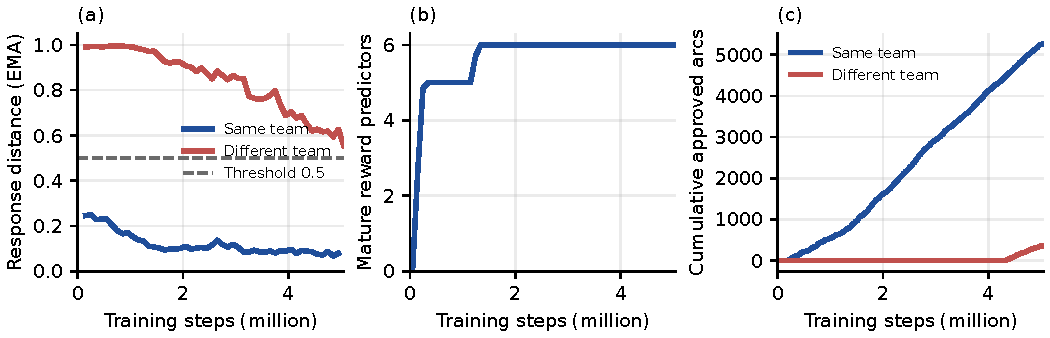
\includegraphics[width=.98\textwidth]{../figures/discovery_log.pdf}
\caption{창고 과제의 팀 발견(모서리 목적지, 개인 보상, seed 1, 5M step). (a) 비교한 쌍의 응답 거리 EMA 평균, 100k step 구간. 점선은 승인 문턱이다. (b) 보상 예측기가 성숙한 에이전트 수. (c) 실제 관계별 방향 있는 팀원 접근 arc 누적.}\label{fig:gate-data}
\end{figure*}

\subsection{팀 관계가 팀원 가치에 중요한 이유}
팀원의 Critic은 팀원에게만 쓸모 있을까? 저장된 독립 PPO checkpoint로 반사실 점검을 했다. 같은 환경 상태에서 뒤처진 에이전트를 자기 정책으로, 또는 다른 에이전트의 정책으로 움직이게 했다. 나머지 에이전트는 자기 정책을 유지했다. 그리고 100 step 동안 뒤처진 에이전트 자신의 return을 비교했다(공통 난수, 8회 반복). 네 checkpoint 데이터(한 학습의 두 시점, 좌표가 보이는 이전 설정의 두 학습)에서, 같은 팀 Critic이 뒤처진 에이전트에 대해 0.2보다 큰 상승을 예측했을 때 그 팀원의 정책은 실제로 에이전트의 return을 67--100\%의 경우에 높였다(평균 이득 0.28--0.58). 비슷한 크기의 다른 팀 상승은 평균 이득이 $-0.01$--$0.14$에 그쳤다. 앞선 에이전트에게는 다른 팀 Critic이 상승을 예측하는 경우가 많았지만, 실제로는 유의한 손실이 따르기도 했다. 예측 상승은 실제 이득을 최대 1.6배까지 과대평가했다. 이 관찰은 발견 단계와 상승분의 보수적 축소가 모두 필요하다는 근거다.

\subsection{학습 성능}
그림~\ref{fig:baseline}은 처음부터 학습한 독립 PPO 기준선(seed 2개)이다. 5M step 뒤 평가 episode당 배송 25.7과 24.1에 이르며, 학습 진행은 에이전트마다 고르지 않다. 통합 PGCT 비교(표~\ref{tab:pending})는 진행 중이며 진행 중으로 표시한다. 중간 곡선은 싣지 않는다.

\begin{figure}[t]\centering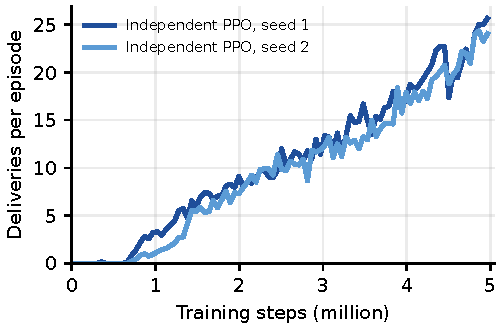
\includegraphics[width=\columnwidth]{../figures/baseline_ippo.pdf}
\caption{처음부터 학습한 독립 PPO: 500 step episode당 평가 배송 수(모서리 목적지, 개인 보상).}\label{fig:baseline}\end{figure}

\begin{table}[t]\centering\small
\begin{tabular}{lcc}\toprule
방법(분기, +0.5M) & 뒤처진 에이전트 & 앞선 에이전트\\\midrule
독립 PPO & \pending & \pending\\
정답 팀 Max-GAE & \pending & \pending\\
정답 팀, 성숙만 & \pending & \pending\\
PGCT & \pending & \pending\\
수를 맞춘 무작위 & \pending & \pending\\\bottomrule
\end{tabular}
\caption{공통 1.024M step checkpoint에서 분기한 뒤의 평가 배송 수(seed 1, 3, 5). 학습이 끝나면 결과를 넣는다.}\label{tab:pending}\end{table}

\section{한계}
발견은 보상 경험에 의존한다. 자격 있는 보상을 한 번도 받지 못한 에이전트는 짝지을 수 없고, 그 에이전트가 바로 도움이 가장 필요한 에이전트일 수 있다. 우리 checkpoint에서는 뒤처진 세 에이전트 가운데 둘이 배송이나 반납 사건이 없었다. 그래서 정답 팀 방법은 이들을 돕지만 PGCT는 판정을 보류한다. probe는 경험한 사건만 다루며, 좌우 대칭은 예측이 대칭 장면으로 일반화된다고 가정한다. 5M 학습 후반에는 다른 팀 거리가 내려가고 다른 팀 승인이 일부 나타났으며, 원인은 아직 분석하지 않았다. 팀원 Critic은 팀원 자신의 정책과 이력 분포에서 return을 추정하므로, 다른 에이전트의 이력에서 계산한 값은 편향될 수 있고 최댓값이 그 편향을 키울 수 있다. 크기 축소는 Actor 섭동을 제한하지만 도움이 된다는 증명은 아니다. 1{,}024 step rollout에서는 거의 모든 쌍이 한 번 이상 만나므로, 접촉 규칙은 주로 승인이 쌓이는 속도를 제한한다. 마지막으로, 현재 근거는 한 환경 계열과 적은 seed에서 나왔다.

\section{결론}
PGCT는 개인 보상 응답으로 잠재 팀원을 온라인에서 찾는다. 각 에이전트는 자기 보상을 예측하고, 만난 팀원과 공개 보상 사건 probe에서 예측을 비교하며, 충분한 자기 경험으로 뒷받침되는 지속적 일치만 승인한다. 발견한 관계는 보수적으로 쓴다. 승인된 팀원의 Critic이 마스크와 크기 제한을 둔 Max-GAE 항으로 Actor advantage를 바꾸고, 각 Critic은 자기 return을 유지한다. 두 팀 창고 과제에서 발견은 이른 시점에 팀원을 구분하고 팀원 접근의 대부분을 실제 팀원에게 보낸다. 이 접근이 학습을 빠르게 하는지는 진행 중인 분기 비교로 검증하고 있다.

\bibliographystyle{plainnat}
\bibliography{../references}

\appendix
\section{구현 세부}
발견 상태의 일관성을 검사한다. rollout 시작 스냅샷과 비교 사이에 예측기가 다시 학습되면 오류로 처리한다. 승인은 저장된 round와 EMA 값에서 다시 구성하며, 현재 성숙 표시와 대조한다. 자기 rollout에서 explained variance가 문턱보다 낮은 donor Critic을 제외하는 선택 필터가 있지만, 문턱을 정하지 않았으므로 꺼 두었다. donor 집합은 update 한 번 동안 고정된다. 자기 return 목표는 Actor advantage를 만들기 전에 계산한다.

근거 자료: 발견 로그는 \path{runs/acv2_s1_20261029_084340}, 독립 PPO 기준선은 \path{runs/ac_20261023_185556}(seed 1, 2), 분기 비교는 \path{runs/maxgae_br1M_20261102_165216}이다. 그림은 원본 로그에서 \path{output/pgct_docs_20261102/evidence_plots.py}로 다시 만든다.
\end{document}
